\chapter{Seguimiento}
En esta secci�n hablaremos sobre el seguimiento del proyecto, que se hizo basandose en la metodolog�a SCRUM (como el resto del TP). SCRUM prevee un tipo de reuni�n de seguimiento: la daily stand-up meeting. 

Nosotros hicimos este tipo de reuni�n informal y r�pida mas o menos constantemente a lo largo de este mes. En realidad no lo hicimos porque la metodolog�a as� lo prevee (de hecho no las hicimos todos los d�as) sino porque es algo que nos surge naturalmente del trabajo en equipo en otras materias tambi�n (hace varios a�os que hacemos grupo juntos, si bien no siempre exactamente el mismo, todos nos conociamos de antes). Tambi�n hicimos una reuni�n con nuestro corrector, pero esa se desvi� un poco por la presencia del mismo (aprovechamos para hacerle consultas y mostrarle lo que teniamos).

Periodicamente fuimos actualizando el \textit{taskboard}, no en un pizzar�n f�sico, en un archivo en nuestro repositorio. En �l ibamos cambiando el estado de las tareas y de las stories cuando era necesario: Sin empezar, en progreso, tarea terminada. Tambi�n ibamos actualizando la cantidad de horas que faltaban para terminar el proyecto. Estas horas fueron el input para armar el \textit{burndown chart}.

\begin{figure}[h]
\centering
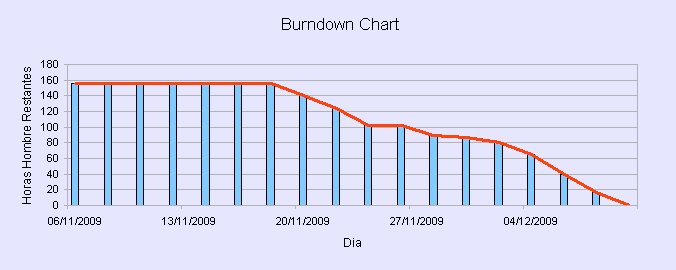
\includegraphics[scale=0.4]{./figuras/burnDown.png}
\caption{Burn Down Chart}
\end{figure}

En el burndown chart, se puede apreciar cuantas horas esfuerzo faltan para terminar el sprint. (Se puede ver esto discriminado por tareas en la tabla). Podemos ver que al pricipio, las horas esfuerzo se mantuvieron constantes. 

Hay dos motivos esenciales para ello: por un lado, en las stories no est�n incluidas las meta-tareas, como por ejemplo armar el product y sprint backlog, escribir los casos de aceptaci�n, o empezar a escribir este informe.

Por otro lado, al principio del trabajo pr�ctico teniamos dudas (que iban surgiendo a medida que haciamos las distintas partes del trabajo) que nos frenaban. Una vez que ya sab�amos exactamente que ten�amos que hacer y nos ibamos distribuyendo el trabajo espontaneamente, el ritmo de trabajo fue mayor (adem�s por la misma inercia de tener el trabajo empezado).

Los obst�culos que tuvimos fueron mas que nada temporales: la presencia del parcial de esta y de otras materias hizo que bajaramos la cantidad de horas dedicadas al trabajo pr�ctico, pero logramos no frenar del todo el desarollo de mismo. 

Los otros obst�culos que tuvimos fue en la implementaci�n: en la primera parte del trabajo estabamos muy contentos de haber hecho r�pidamente la implementaci�n en un lenguaje de programaci�n que ninguno dominaba. Esta vez, hubo alguno errores que nos dieron dolores de cabeza y nos hicieron pensar durante rato, pero todos fueron resueltos.

En general, estamos contentos con como se desaroll� el trabajo pr�ctico. Si bien no llegamos con tanto tiempo de sobra como hubieramos querido, es comprensible dado que tuvimos varias restricciones temporales (TPs y parciales de otra materia, la mitad del grupo trabaja) que hicieron que no pudieramos terminarlo antes.
\begin{landscape}
\begin{figure}[h]
\centering
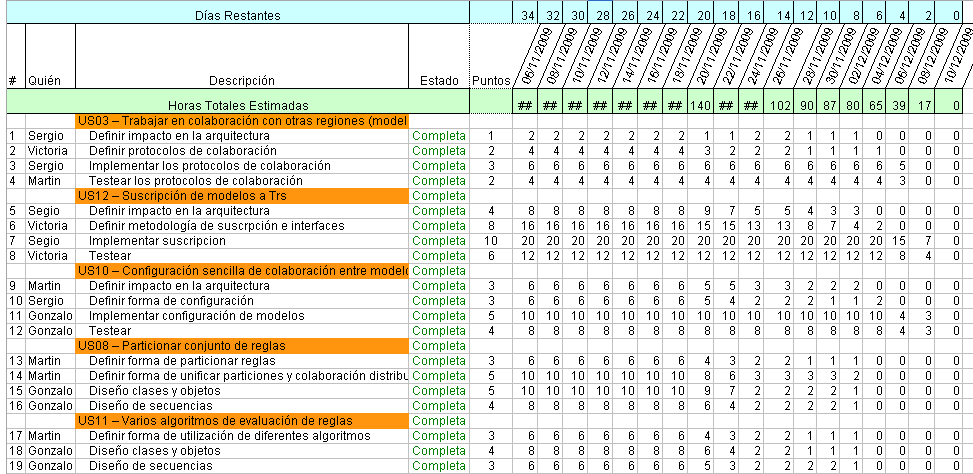
\includegraphics[scale=0.7]{./figuras/taskboard.png}
\caption{Taskboard}
\end{figure}
\end{landscape}  